For the present study 227 existing roll decay model tests conducted at SSPA Maritime Dynamics Laboratory are used. The roll decay test are conducted by forcing the model to an initial roll angle and then release it to oscillate freely in six degrees of freedom. The tests are conducted either  at zero speed or at speed with a fixed rudder angle. The scaled ship models are between 3 and 6 meters of length. The measurement accuracy of these model tests is very good. When time series from 20 sets of repeated tests were investigated the average $R^2$ was 0.995. The tests were originally conducted in commercial projects for new buildings of merchant ships. The main parameters and ship types of the ships are summarized in Appendix \ref{app:ships}. 

The roll decay test database is used to build a roll damping database. The parameter identification technique was used to extract damping coefficients from the roll decay tests. It was investigated whether the linear model (equation \ref{eq:roll_decay_equation_himeno_linear}), quadratic model (equation \ref{eq:roll_decay_equation_himeno_quadratic_b}) or cubic model (equation \ref{eq:roll_decay_equation_cubic}) was best suited  to build the roll damping database . Simulations with the three mentioned models were conducted and the accuracy of the fit was evaluated with the $R^2$ score coefficient, based on model test and simulation time series.
The average $R^2$ was 0.995 for the cubic model, 0.993 for the quadratic and 0.986 for the linear model. Since the quadratic model has almost the same accuracy as the cubic model it was selected to be used for the roll damping database. Figure \ref{fig:roll_decay_model_compare} shows a comparison between the models for one of the roll decay test. It can be seen that the linear model can not give a perfect representation for the whole range of roll angles.

\begin{figure}[H]
    \centering
    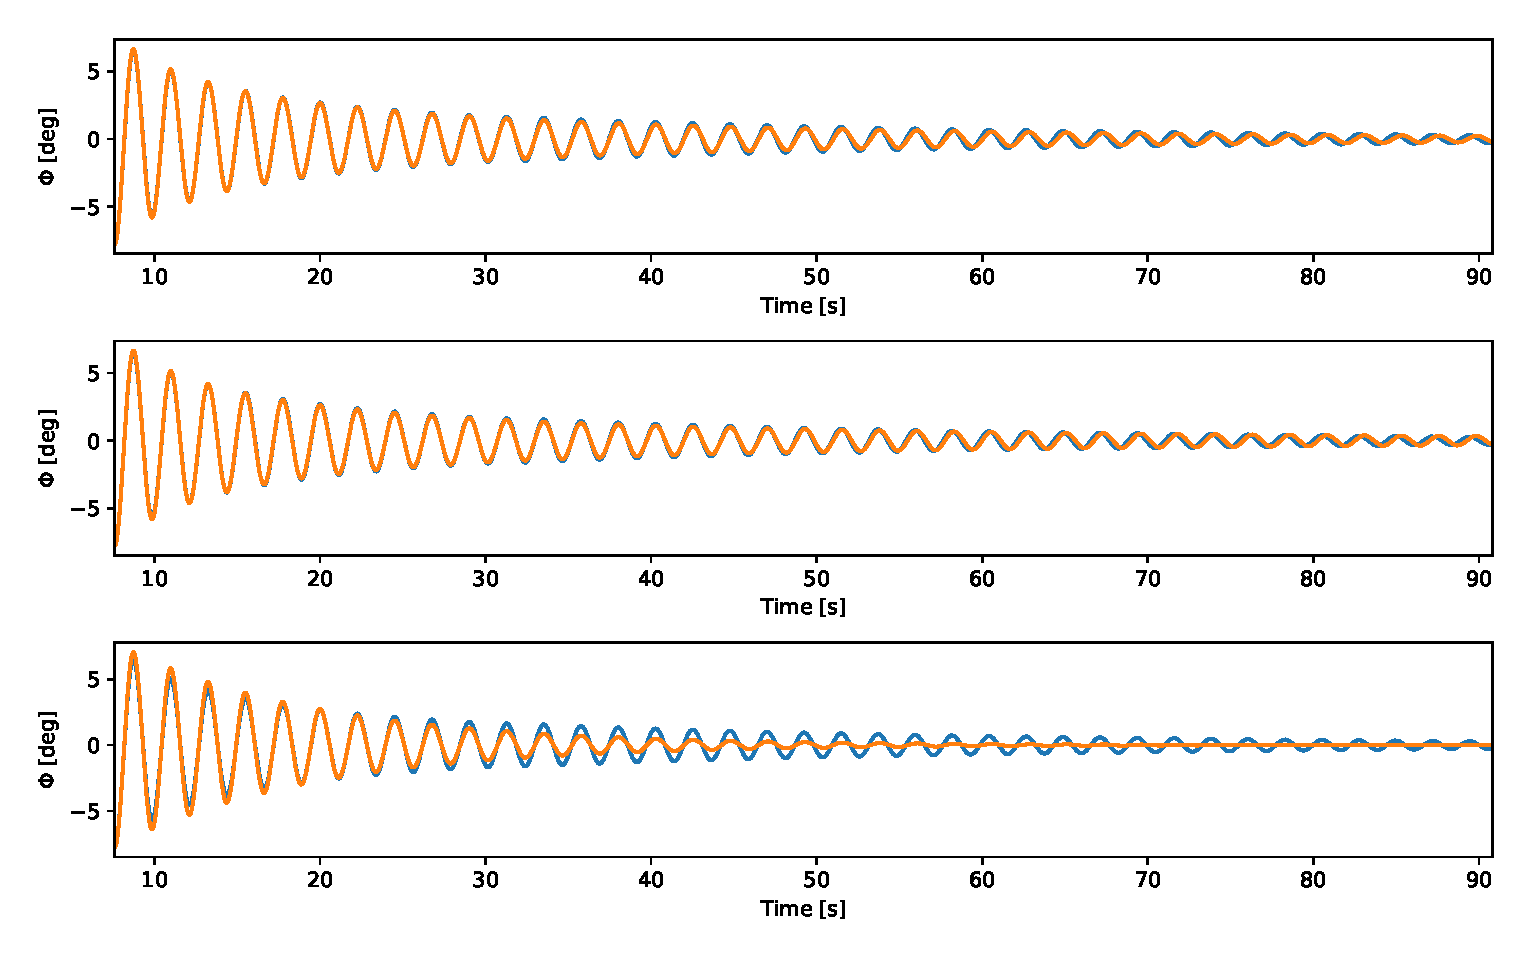
\includegraphics[width=12cm, height = 6cm ]{figures/roll_decay_model_compare.eps}
    \caption{Roll decay test comparison of linear, quadratic and cubic model}
    \label{fig:roll_decay_model_compare}
\end{figure}

